\documentclass[25pt, 
               a0paper, 
               portraitmargin = 0mm, 
               margin = 0mm,
               innermargin = 50mm,
               blockverticalspace = 8mm,
               colspace = 40mm,
               subcolspace = 8mm]
               {tikzposter}

%%%%% packages %%%%%
\usepackage[utf8]{inputenc}
\usepackage{wrapfig}
\usepackage{enumitem}



\usetikzlibrary{positioning,calc}

\usepackage{subfig}
\usepackage{booktabs}
\usepackage{float}
\usepackage{array}
\usepackage[flushleft]{threeparttable}

\newcommand*{\affmark}[1][*]{\textsuperscript{#1}}

\captionsetup[subfloat]{justification=RaggedRight,singlelinecheck=off}

\newcolumntype{L}[1]{>{\raggedright\let\newline\\\arraybackslash\hspace{0pt}}m{#1}}
\newcolumntype{C}[1]{>{\centering\let\newline\\\arraybackslash\hspace{0pt}}m{#1}}
\newcolumntype{R}[1]{>{\raggedleft\let\newline\\\arraybackslash\hspace{0pt}}m{#1}}

%itemize
\setitemize{labelindent=1.5em,labelsep=1em,leftmargin=*}
\setenumerate{labelindent=1.5em,labelsep=1em,leftmargin=*}


%%%%% remove inner sep within fbox
\setlength{\fboxsep}{0pt}%
\setlength{\fboxrule}{1pt}%

%%%%% Remove “LaTeX Tikzposter” in bottom right corner
\tikzposterlatexaffectionproofoff

%%%%% Font family
\renewcommand{\familydefault}{\sfdefault}


%%%%% layout %%%%%
\definecolor{b-it_blue}{HTML}{016ABA}
\definecolor{b-it-bots_blue}{HTML}{0071BD}
\definecolor{brsu_blue}{HTML}{0BA1E2}
\definecolor{mas-group_dark-blue}{HTML}{0072bb}
\definecolor{mas-group_light-blue}{HTML}{2889c7}
\definecolor{mas-group_cyan}{HTML}{42a3e1}
\definecolor{mas-group_light-gray}{HTML}{dcdcdc}
\definecolor{mas-group_dark-gray}{HTML}{8c8c8c}


% color scheme
\usetheme{Simple}
\definecolorstyle{BrsuColorStyle}
{
	\definecolor{colorOne}{named}{white}
	\definecolor{colorTwo}{named}{black}
	\definecolor{colorThree}{named}{b-it_blue}
}
{
	\colorlet{backgroundcolor}{colorOne}
	\colorlet{framecolor}{colorOne}	
	\colorlet{titlefgcolor}{colorThree}
	\colorlet{titlebgcolor}{colorOne}
	\colorlet{blocktitlebgcolor}{colorOne}
	\colorlet{blocktitlefgcolor}{brsu_blue}
	\colorlet{blockbodybgcolor}{colorOne}
	\colorlet{blockbodyfgcolor}{colorTwo}
}
\usecolorstyle{BrsuColorStyle}


% blocks
\defineblockstyle{BrsuBlockStyle}
{
	titlewidthscale=1.0, 
	bodywidthscale=1.0,
	titleleft,
	titleoffsetx=-5mm,
	titleoffsety=0mm,
	bodyoffsetx=0mm,
	bodyoffsety=0mm,
	bodyverticalshift=8mm,
	roundedcorners=0,
	linewidth=0pt,
	titleinnersep=5mm,
	bodyinnersep=0mm
}{
	\draw[color=framecolor, fill=blockbodybgcolor, rounded corners=\blockroundedcorners] (blockbody.south west) rectangle (blockbody.north east);
	\ifBlockHasTitle
		%\draw[color=framecolor, fill=blocktitlebgcolor, rounded corners=\blockroundedcorners] (blocktitle.south west) rectangle (blocktitle.north east);
		\draw [dash pattern=on 5pt off 10pt, color=brsu_blue, line width = 2mm] (blockbody.north west) -- (blockbody.north east);	
	\fi
}
\useblockstyle{BrsuBlockStyle}


%%%%% title %%%%%
\title{\parbox{0.85\linewidth}{Predicting Object Locations using Spatio-Temporal
Information by a Domestic Service Robot: A Bayesian
Learning Approach}}
\author{\parbox{0.85\linewidth}{Deebul Nair\affmark[1], Tim Niemueller\affmark[2], Paul G. Pl\"{o}ger\affmark[1],  Gerhard Lakemeyer\affmark[2]}}
\institute{\affmark[1]Bonn-Rhein-Sieg University of Applied Sciences, Germany \\\affmark[2]Rheinisch-Westfalische Technische Hochschule Aachen University, Germany}
\date{\today}

% format title
\definetitlestyle{BrsuTitle}{linewidth = 0mm,
							innersep = 0pt,
							titletotopverticalspace = 2.5cm,
							titletoblockverticalspace = 0cm
}{
	\begin{scope}[line width=0pt]
		\draw[color=blocktitlebgcolor, fill=titlebgcolor]
		(\titleposleft,\titleposbottom) rectangle (\titleposright,\titlepostop);
	\end{scope}
}
\usetitlestyle{BrsuTitle}

\settitle
{
	\vbox
	{
		\color{titlefgcolor} {\bfseries \Huge \sc \textbf{\@title} \par}
		\vspace*{1em}
		{\LARGE \@author \par}
		\vspace*{1em} 
		{\large \textit{\@institute}}
	}
}


\begin{document}

\maketitle[width=0.88\textwidth]

%%%% LAYOUT BLOCK
\block{}
{
\begin{tikzpicture}[remember picture,overlay]
\pgfmathsetmacro\barwidth{2.86}
\pgfmathsetmacro\topbarlength{13}


% left side
\node at (current page.north west) {\draw [fill=b-it_blue, draw=b-it_blue] (-0.14,0) rectangle (\barwidth, -\topbarlength);};
\node at (current page.north west) {\draw [fill=brsu_blue, draw=brsu_blue] (-0.14,-14) rectangle (\barwidth,-110);};  \node at (current page.south west) {\draw [fill=mas-group_dark-gray, draw=mas-group_dark-gray] (-0.14, 8) rectangle (\barwidth, 0);};
    
% top right
\node at (current page.north east) {\draw [fill=b-it_blue, b-it_blue] (-0.36,0) rectangle (-3.36,-\topbarlength);};
\node at (current page.north east) {\draw [fill=brsu_blue, brsu_blue] (-4.36,0) rectangle (-7.36,-\topbarlength / 4 * 3);};
\node at (current page.north east) {\draw [fill=mas-group_dark-gray, mas-group_dark-gray] (-8.36,0) rectangle (-11.36,-\topbarlength / 4 * 2);};
\node at (current page.north east) {\draw [fill=mas-group_light-gray, mas-group_light-gray] (-12.36,0) rectangle (-15.36,-\topbarlength / 4);};
	
\end{tikzpicture}
}

 %\vspace{1cm}
\begin{columns}
%%%%% LEFT COLUMN %%%%%%%%%%%%%%%%%%%%%%
    \column{0.5}
   
    \block{Motivation}	
    {
One of the ways domestic service robots can better assist humans is by providing
personalized, predictive and context-aware services. Robots can observe human
activities and work patterns and provide time-based contextual assistance. This
thesis aims to enable domestic robots to empirically learn about human behaviour
and preferences. In the current literature, user preferences are learned for a generic home environment, on the contrary we learn preferences over a specific home. The developed approaches in this thesis
cover the following two knowledge generation topics: 
\begin{itemize}
	\item learning user preferences in object placement
	\item learning user location preferences
\end{itemize}
        \begin{tikzfigure}[Robot recording  different locations of the cup.]
            %\includegraphics[width=\linewidth]{images/cup/introduction.jpg}
	        %\\ \vspace{2.5mm}
		    \includegraphics[width=0.243\linewidth]{images/cup/cup_cupboard.jpg}
		    \includegraphics[width=0.243\linewidth]{images/cup/cup_dishwasher.jpg}
		    \includegraphics[width=0.243\linewidth]{images/cup/cup_on_table.jpg}
		    \includegraphics[width=0.243\linewidth]{images/cup/cup_sink.jpg}
	    \end{tikzfigure}
    }
    
    \block{Approach}
    {
    Robots generate a lot of information using the raw data from their sensors,
which is often discarded after use. If this information is recorded, it can be used to generate new knowledge\cite{niemueller2012generic}. The thesis proposes models to generate knowledge about user preferences using stored information in the robot memory. 
    
    \begin{tikzfigure}[Knowledge Pyramid]
		    \includegraphics[width=0.8\linewidth]{images/dikw-pyramid.png}
	\end{tikzfigure}
    
    }
    


    %%%%% RIGHT COLUMN %%%%%%%%%%%%%%%%%%%%%%
   
    
    \block{Bayesian Machine Learning }
	{
	    \begin{itemize}
	        \item Human behaviour and preferences are based on time of the day.
	        \item The problem of learning preferences from previous information in robot memory, is formulated as a Bayesian inference problem
            \begin{equation}
	            p (\theta | D , t) = \frac{p (t | \theta , D) p (\theta | D )}{p (D)}
            \end{equation}
where $\theta$ represents the user preferences, $t$  represents the time of the day and $D$ represents the previous information of the object location or the person location.
        \end{itemize}

	  
	  \begin{tikzfigure}[Probability distribution of user preference in placing cup at different locations.]
		    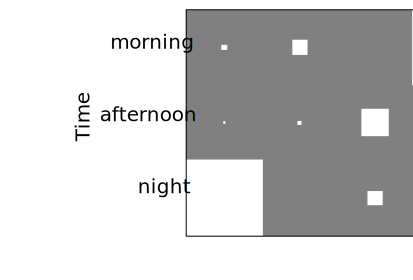
\includegraphics[width=0.6\linewidth]{images/absent_groundtruth.png}
	  \end{tikzfigure}
      
	
    }
    
    
     \column{0.5}
     
	\block{Probabilistic Graphical Models } % continuation of Features block
	{

           Based on the problem type and the input datatype, different models were developed to represent the user preferences.
    	   Bayesian models are represented using probabilistic graphical models.
        \begin{itemize}
            \item\textbf{ Hierarchical Beta Bernoulli model (HBB)}
        \end{itemize}	
          
       \begin{minipage}{0.4\linewidth}     

       \begin{tikzfigure}  
          \def\svgwidth{0.5\linewidth} \input{HBM.pdf_tex}  
       \end{tikzfigure}
        \end{minipage}
        \hspace{5.5cm}
        \vrule{}
        \hspace{-1.5cm}
        \begin{minipage}{0.6\linewidth}
        \begin{itemize}
        	\item modelling \textbf{single} location \\ preference.
	        \item data type is \textbf{boolean}.
\end{itemize}
        \end{minipage}


    \begin{itemize}
                \item \textbf{Hierarchical Dirichlet Categorical model (HDC)}
    \end{itemize}	

       \begin{minipage}{0.4\linewidth}     
       \begin{tikzfigure}  
          \def\svgwidth{0.4\linewidth} \input{HDM.pdf_tex}  
       \end{tikzfigure}
        \end{minipage}
        \hspace{5.5cm}
        \vrule{}
        \hspace{-1.5cm}
        \begin{minipage}{0.6\linewidth}
        \begin{itemize}
        	\item modelling \textbf{multiple} location \\ preferences.
	        \item data type is \textbf{discrete} categories.
\end{itemize}
        \end{minipage}
           \break
          The models were implemented using \textbf{Probabilistic Programming languages} BayesPy \cite{luttinen_bayespy_2014} and PyMC3 \cite{salvatier2016probabilistic}

	}

    \block{Results}
	{
	\begin{itemize}
	\item The HBB model was evaluated on \textbf{KTH dataset}\cite{krajnik_wheres_2015}, which contained
locations of 37 objects in an office for a duration of 5 weeks, collected by a mobile robot. The learning on this dataset showed the model could predict locations of 26 objects with 70\% accuracy. 
    \item The HBB model was evaluated on a \textbf{Brayford dataset} \cite{krajnik_wheres_2015} which contained human presence information of 6 locations in an office, collected by a mobile robot. Evaluation results showed that the robot was able to learn with more than 60\% accuracy for all the rooms.
    \item HDC model for learning the user location preferences was evaluated in the \textbf{Aruba dataset}\cite{aruba}. The evaluation results showed that the model was consistently predicting user location with 63\% accuracy. 
\end{itemize}
        
	
	}   % end results block
	
	
    \block{Conclusions}
	{
	\begin{itemize}

    \item  The Bayesian models were able to learn user preferences to a large extent. Regular patterns were learned, while objects/persons that followed no observable pattern were not predicted well.  
\item We hope that our approaches will set up service
robots into the existing household by knowing what and who are there in a home and adapting to them. 
    \item   These service robots will grow and change with the users, with a greater awareness
of the world around them.
\end{itemize}
	}
    
    \block{References}
    {
		\small
            
            \nocite{niemueller2012generic}
            \nocite{luttinen_bayespy_2014}
            \nocite{salvatier2016probabilistic}
            \nocite{krajnik_wheres_2015}
            \nocite{aruba}
            
    		\begingroup
			\renewcommand\refname{\vskip -2cm}
	    		\bibliography{literature_references}
			\bibliographystyle{plain}
		\endgroup
    }
    
    \block{Acknowledgements}
    {
    		\small
		We gratefully acknowledge the continued support by the b-it Bonn-Aachen International Center for Information Technology, Rheinisch-Westfalische Technische Hochschule Aachen University and the Bonn-Rhein-Sieg University of Applied Sciences.
    }
    
   
\end{columns}


%%%%% FOOTER %%%%%%%%%%%%%%%%%%%%%%
\block{}
{
\begin{tikzpicture}[remember picture,overlay] 

	\node [shift={(-11cm, 4cm)}] at (current page.south) {\includegraphics[height=4cm]{gfx/b-it.pdf}};
	\node [shift={(11cm, 4cm)}] at (current page.south) {\includegraphics[height=4cm]{gfx/brsu.eps}};
	\end{tikzpicture}
}

 
\end{document}

